% listing of script
\lstinputlisting[style= Matlab-editor,basicstyle = \mlttfamily,
  caption=Exercise 5 script]{Week_2_master/exercise5.m}


% tabulated separation locations
\begin{table}[H]
\centering
\begin{tabular}{c|c}
\hline
Re                    & \multicolumn{1}{c}{x/L} \\ \hline
$10^6$ & 0.016                   \\
$10^7$ & 0.985                   \\
$10^8$ & No Separation                       \\ \hline
\end{tabular}
\caption{Separation locations for varied $Re_L$ at velocity gradient = -0.50}
\end{table}

\begin{table}[H]
\centering
\begin{tabular}{c|c}
\hline
$\frac{d(u_e/U)}{d(x/L)}$ & \multicolumn{1}{c}{x/L} \\ \hline  
-0.25 & No Separation     \\
-0.5  & 0.985 \\
-0.95 & 0.505 \\ \hline
\end{tabular}
\caption{Separation locations for varied velocity gradient at $Re_L = 10^7$}
\end{table}

\begin{figure}[H]
\centering
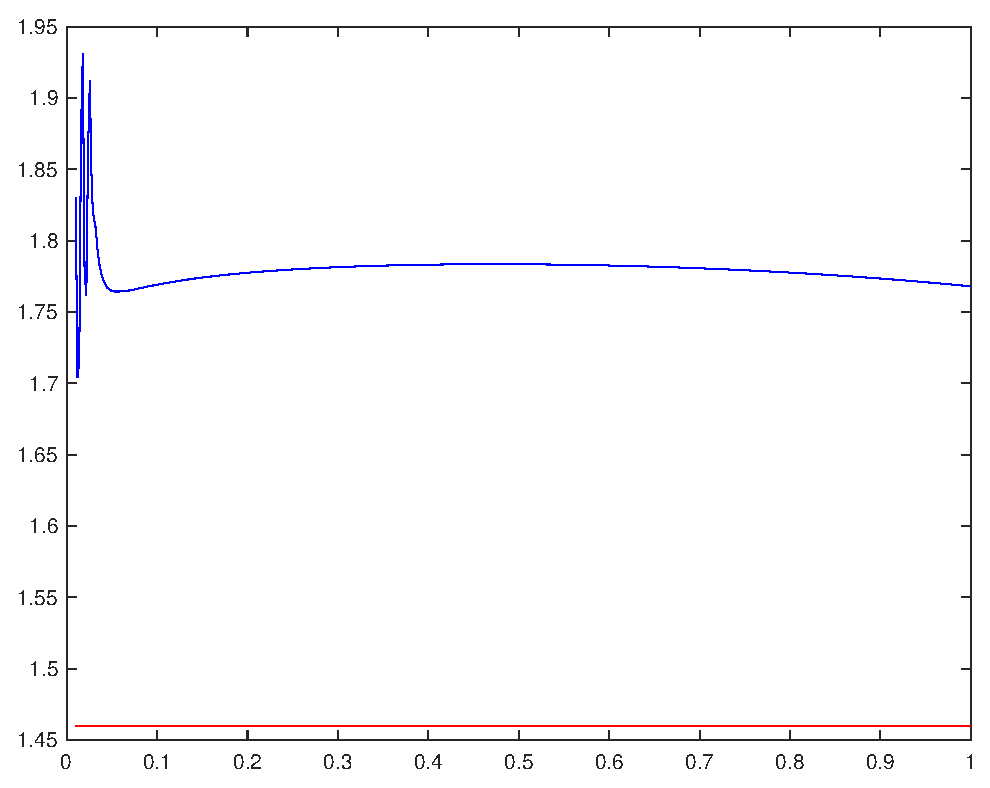
\includegraphics[scale=0.76]{graphs/e5g1.eps}
\caption{Dimensionless boundary layer thickness plot for $Re_L = 10^7$ and velocity gradient = -0.50 }
\label{e1g1}
\end{figure}

